% !TEX root = main.tex

\section{并发控制} % Chap 15
\subsection{基于锁的协议}
\begin{itemize}
	\item 共享锁(shared):如果事务$T_i$获得了数据项$Q$上的共享型锁(记为$S$),则$T_i$\textbf{可读但不能写}$Q$
	\item 排他锁(exclusive):如果事务$T_i$获得了数据项$Q$上的排他型锁(记为$X$),则$T_i$既\textbf{可读又可写}$Q$
\end{itemize}

若某个事务请求的锁与其他事务持有的锁相容,它才可以被授予锁;否则等待所有不相容锁释放。
\begin{table}
\centering
\caption{锁相容性矩阵comp}
\begin{tabular}{|c|c|c|}\hline
 & $S$ & $X$\\\hline
$S$ & true & false\\\hline
$X$ & false & false\\\hline
\end{tabular}
\end{table}

容易发生如下死锁
\begin{figure}[H]
\centering
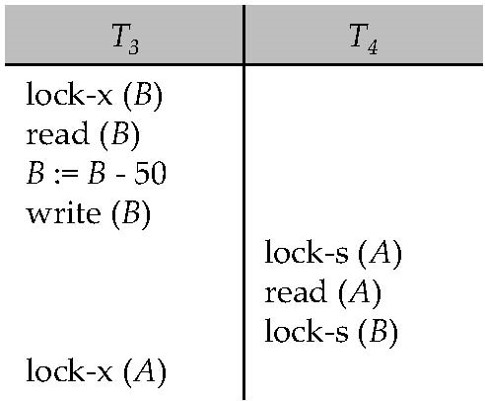
\includegraphics[width=0.3\linewidth]{fig/deadlock.jpg}
\end{figure}

令$\{T_0,\ldots,T_n\}$是参与调度$S$的一个事务集,若存在数据项$Q$,使得$T_i$在$Q$上持有$A$型锁,之后$T_j$在$Q$上持有$B$型锁,且$comp(A,B)=false$,则称在$S$中$T_i$先于$T_j$,记为$T_i\to T_j$,即在任何等价的串行调度中,$T_i$必须出现在$T_j$之前。

两阶段封锁协议:可保证冲突可串行化,但不能保证不发生死锁,对于\textbf{每个事务}有以下两个阶段
\begin{enumerate}
	\item 增长(growing)阶段:事务可以获得锁,但不能释放锁(也包括锁的升级,共享$\to$排他)
	\item 缩减(shrinking)阶段:事务可以释放锁,但不能获得新锁(也包括锁的降级,排他$\to$共享)
\end{enumerate}

\begin{figure}[H]
\centering
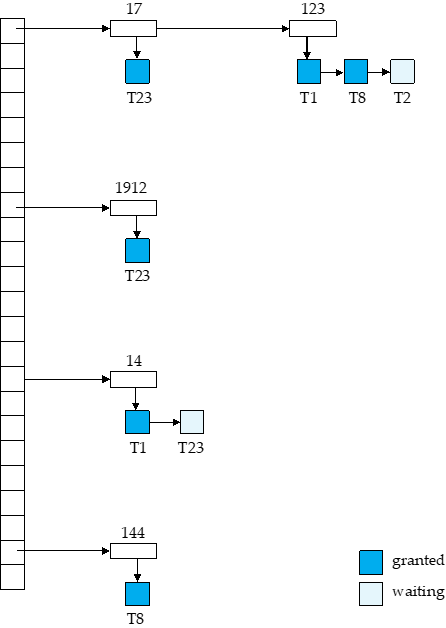
\includegraphics[width=0.4\linewidth]{fig/lock_table.png}
\end{figure}

自动为事务产生适当的加锁、解锁指令:
\begin{itemize}
	\item 事务$T_i$进行$read(Q)$操作时,系统产生一条$lock-S(Q)$指令,该$read(Q)$指令紧跟其后
	\item 事务$T_i$进行$write(Q)$操作时,系统检查$T_i$是否已在$Q$上持有共享锁。
	若有,则系统发出$upgrade(Q)$指令,后接$write(Q)$指令。
	否则系统发出$lock-X(Q)$指令,后接$write(Q)$指令。
	\item 当一个事务提交或中止后,该事务持有的所有锁都被释放。
\end{itemize}

\subsection{基于图的协议}
要求所有数据项集合$D=\{d_1,d_2,\ldots,d_n\}$满足偏序$\to$:如果$d_i\to d_j$,则任何既访问$d_i$又访问$d_j$的事务必须首先访问$d_i$,然后访问$d_j$。
偏序意味着集合$D$可以视为有向无环图,称为数据库图。
\begin{figure}[H]
\centering
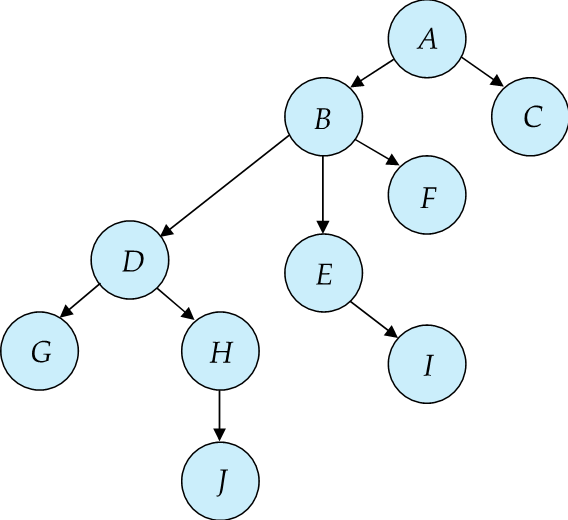
\includegraphics[width=0.4\linewidth]{fig/tree_protocol.png}
\end{figure}

在树形协议中,可用的加锁指令只有lock-X。
每个事务$T_i$对一数据项最多能加一次锁,并且遵从以下规则:
\begin{enumerate}
	\item $T_i$首次加锁可以对任何数据项进行
	\item 此后,$T_i$对数据项$Q$加锁的前提是$T_i$当前持有$Q$的父项上的锁
	\item 对数据项解锁可以随时进行
	\item 数据项被$T_i$加锁并解锁后,$T_i$不能再对该数据项加锁
\end{enumerate}
所有满足树形协议的调度都是冲突可串行化的,且保证不会发生死锁。

但是不满足可恢复性,而且需要给不需要访问的数据也上锁,增加上锁开销,降低并行程度。

\subsection{死锁处理}
\subsubsection{死锁预防}
\begin{itemize}
	\item 每个事务都要在它执行前锁上它所有要用的数据(预声明)
	\item 强加偏序条件(基于图的协议)
\end{itemize}

更多方法包括:
\begin{itemize}
	\item wait-die机制,非抢占(non-preemptive)技术:老的事务($T_i$时间戳小于$T_j$时间戳,则$T_i$老于$T_j$)会等待年轻的释放数据,年轻的事务不会等待老的事务,直接回滚
	\item wound-wait机制,抢占技术:老的事务强行令年轻事务回滚而不让其等待,年轻事务只能等待老的事务
\end{itemize}

另外还有锁超时(lock timeout)技术,即申请锁的事务至多等待一定时间,若此时间内未授予该事务锁,则事务超时回滚重启。

\subsubsection{死锁检测}
等待(wait-for)图顶点由所有\textbf{事务}组成,边$T_i\to T_j$代表事务$T_i$\textbf{等待}$T_j$释放数据项。
\begin{figure}[H]
\centering
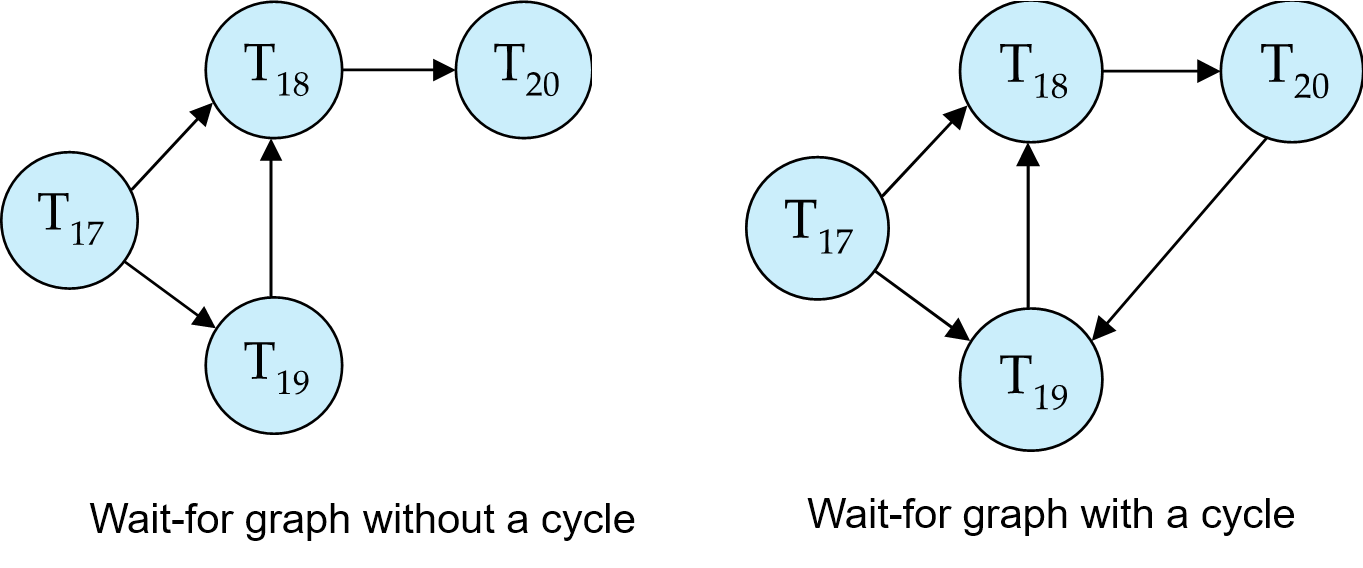
\includegraphics[width=0.6\linewidth]{fig/wait-for_graph.png}
\end{figure}

当事务$T_i$申请的数据项当前被$T_j$持有时,$T_i\to T_j$被插入图中。
只有当事务$T_j$不再持有事务$T_i$所需数据项时,这条边才从等待图删除。

当且仅当等待图存在环时,系统存在死锁。
要检测死锁,系统需要维护等待图,并周期性激活在等待图中搜索环的算法。

\subsubsection{死锁恢复}
通常做的动作有三个:
\begin{itemize}
	\item 选择牺牲者:决定回滚某一最小代价的事务
	\item 回滚:一旦确定回滚事务,则需确定该事务回滚多远,包括彻底回滚和部分回滚
	\item 饿死:如果选择牺牲者主要基于代价,则有可能同一事务总是被选为牺牲者,那该事务始终不能完成任务,就饿死(starvation)了
\end{itemize}

\subsection{基于时间戳的协议}
若事务$T_i$已赋予时间戳$TS(T_i)$,此时有一新事务$T_j$进入系统,则$TS(T_i)<TS(T_j)$,可利用\textbf{系统时钟}或者\textbf{逻辑计数器}实现。
事务的时间戳决定了串行化顺序,因此若$TS(T_i)<TS(T_j)$,则系统必须保证所产生的串行调度等价于事务$T_i$出现在事务$T_j$之前的某个串行调度。

\begin{itemize}
	\item 若$TS(T_i)\geq$W-timestamp(Q),则执行读操作
	\item 若$TS(T_i)\geq$R/W-timestamp(Q),则执行写操作
	\item 其他情况都会导致回滚
\end{itemize}